\begin{flushleft}
	\section{\textcolor{cyan}{Principe de fonctionnement du système de télésurveillance : }}
	\subsection{\textcolor{green}{prototype :}}

	\begin{figure}[h]
		\centering
		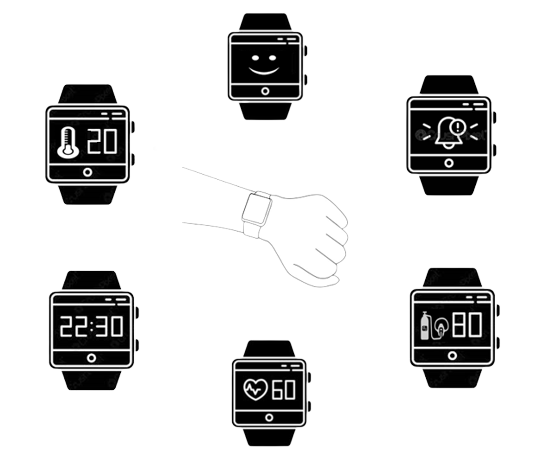
\includegraphics{chapitres/images/System-removebg-preview.png}
		\caption{prototype du système de télésurveillance}
		\label{fig:labelname}
	\end{figure}
	\subsection{\textcolor{green}{Architecture globale du système de télésurveillance :}}
	\begin{figure}[h]
		\centering
		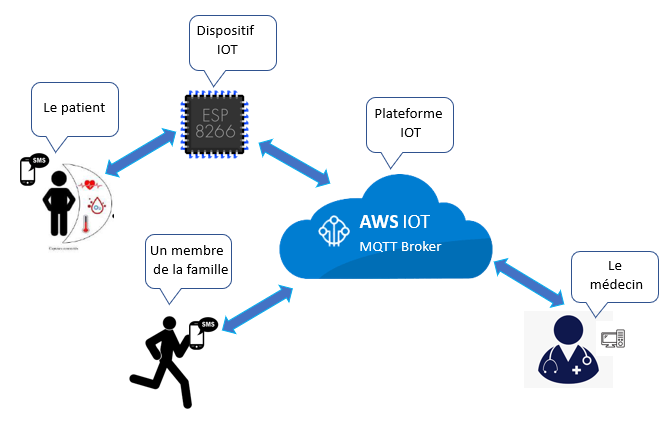
\includegraphics{chapitres/images/architecture.PNG}
		\caption{Architecture complète du système de télésurveillance}
		\label{fig:labelname}
	\end{figure}
	\begin{figure}[h]
		\centering
		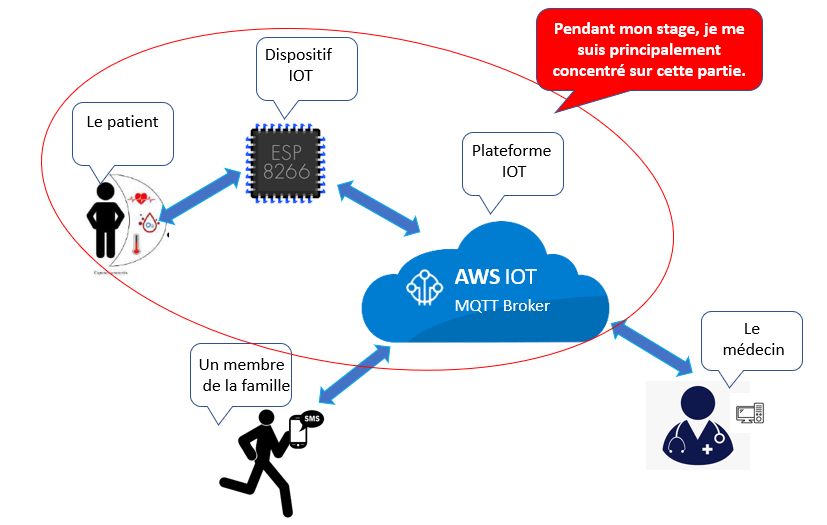
\includegraphics[width=0.9\textwidth]{chapitres/images/architecture1.PNG}
		
	\end{figure}
	\newpage
	\subsection{\textcolor{green}{Description du fonctionnement du système :}}
	Le principe de fonctionnement du système de télésurveillance pour le suivi des patients atteints de maladies cardiaques repose sur l'utilisation d'un dispositif qui mesure la fréquence cardiaque (BPM), la température et la saturation en oxygène (SpO2) du patient. Ce dispositif prend la forme d'une « smartwatch » qui se compose d'un microcontrôleur de type esp8266 et d'un afficheur OLED SSD1306 I2C. Le capteur Max30105 doit être attaché à la main du patient.\newline
	
	Les données mesurées sont envoyées au serveur AWS IoT Core via WiFi. À chaque fois qu'un danger est détecté, le patient reçoit des notifications sur sa smartwatch. Si la situation du patient est très dangereuse, un membre de sa famille reçoit un appel ou un message pour sauver le patient. De plus, le médecin du patient peut suivre en temps réel la situation de son patient.\newline
	\newpage
\end{flushleft}